	Sur la figure ci-dessous :

\begin{itemize}[left=5mm]
	\item les droites (BD) et (CE) sont sécantes en A;
	\item les droites (BC) et (DE) sont parallèles;
	\item $\mathrm{AB}=\np[cm]{6,4}$;\quad
	$\mathrm{AC}= \np[cm]{4,8}$;\quad
	$\mathrm{AD}= \np[cm]{4,8}$;\quad
	$\mathrm{BC}= \np[cm]{8}$.
\end{itemize}
\begin{center}
	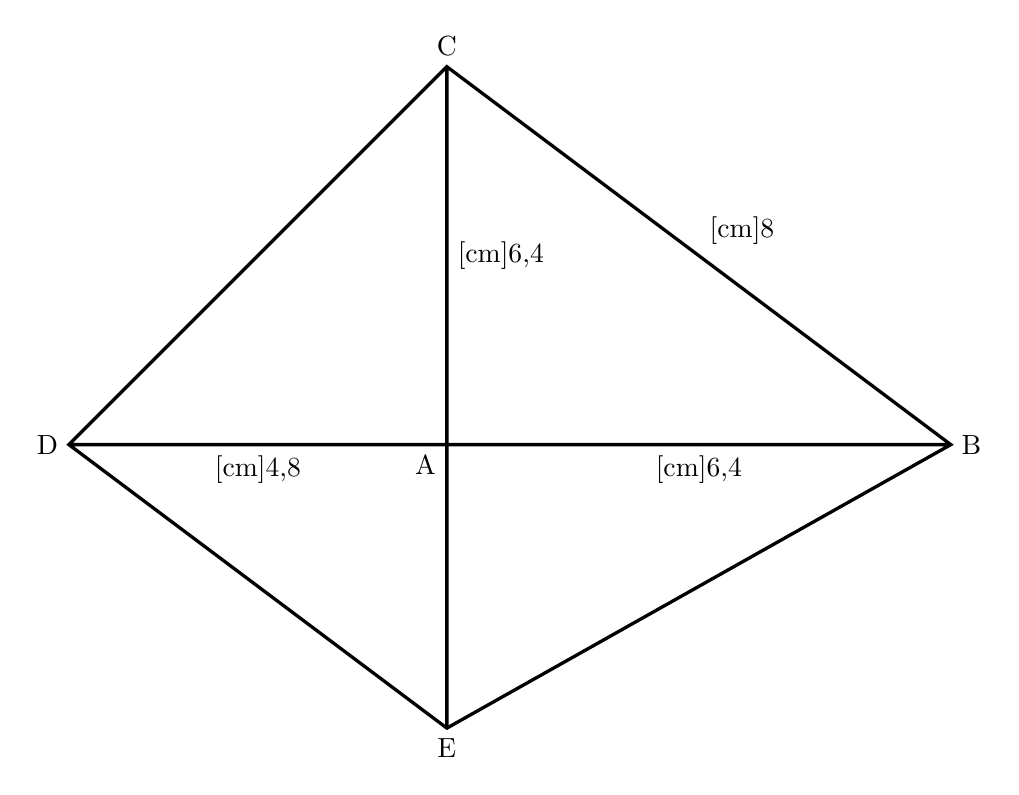
\begin{tikzpicture}[baseline={(0,1.25)}]
		\draw[line width=1.2pt] (0,0)node[below left]{A}
		(6.4,0)node[right]{B}
		-- (0,4.8)node[above]{C} node[pos=0.5,above right]{\np[cm]{8}}
		-- (-4.8,0)node[left]{D}
		-- (0,-3.6)node[below]{E}--cycle
		(6.4,0)--(0,0) node[pos=0.5,below]{\np[cm]{6,4}}
		(-4.8,0)--(0,0) node[pos=0.5,below]{\np[cm]{4,8}}
		(0,4.8)--(0,0) node[pos=0.5,right]{\np[cm]{6,4}}
		(0,-3.6)--(0,0);
	\end{tikzpicture}
\end{center}

\begin{enumerate}
	\item Montrer que le triangle ABC est rectangle en A.

	\item Montrer que $\mathrm{DE}=\np[cm]{6}$ et $\mathrm{AE}= \np[cm]{3,6}$.

	\item Montrer que les angles $\widehat{\mathrm{ABC}}$ et $\widehat{\mathrm{ADE}}$ sont égaux.

	\textbf{Détailler la réponse en précisant la démarche.}

	\item Montrer que les triangles ABC et ADE sont semblables.

	\item Déterminer l'aire du quadrilatère BCDE.
\end{enumerate}


\needspace{10\baselineskip}
% saut de page si moins de 10 lignes disponibles
